\begin{figure}[t]
  \centering
    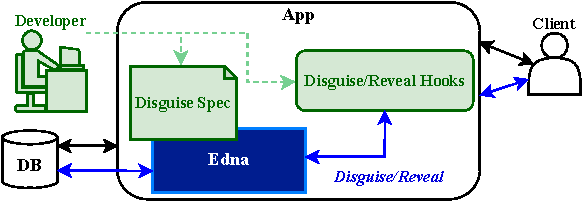
\includegraphics[width=.7\textwidth]{figs/edna_overview}
    \caption[Developers write disguise specifications and add hooks to invoke
    Edna's API.]{Developers write \xx specifications and add hooks to invoke
    \sys from the application (green); in normal operation, clients use these
    hooks in the application to \xx and reveal their data in the database
    (blue).}
  \label{f:edna-overview}
\end{figure}
%

This section introduces the concept of disguised data by describing how
developers and users interact with an application that supports data disguising
and data revealing.
%

%
\sys helps developers realize new options for users to control their data
via \emph{\xxing transformations} and \emph{revealing transformations}.
%
As Figure~\ref{f:edna-overview} shows, a developer integrates an application with \sys by writing \xx specifications
and adding hooks to \xx or reveal data using \sys's API (\S\ref{s:api}). To use \sys, an application does the following:

%
(1) The application registers users with a public--private keypair
that either the application or the user's client generates. \sys stores the
public key in its database, while the user retains the private key for use in
future reveal operations.
%

%
(2) When the application wants to \xx some data, it invokes \sys with the
corresponding developer-provided \xx specification and any necessary
parameters (such as a user ID).
%
\Xx specifications can remove data, modify data (replacing some or all of its
contents with placeholder values), or decorrelate data, replacing
links to users with links to \emph{pseudoprincipals} (fake users generated as
application users with random IDs).
%
% Decorrelation preserves the structure of the application database, and avoids
% integrity issues like dangling foreign keys, while obscuring the data's
% relationship to natural principals (true users).
%
\sys takes the data it removed or replaced and the connections between the user
and any pseudoprincipals it created, encrypts that data with the user's public
key, and stores the resulting ciphertext---the \emph{\xxed data}---such that it
cannot be linked back to the user without the user's
private key.
%

%
(3) When a user wishes to reveal their \xxed data, they pass credentials
to the application, which calls into \sys to reveal the data.
%
Credentials are application-specific: users may either provide their private
key or other credentials sufficient for \sys to re-derive the private key.
%
\sys reads the \xxed data and decrypts it, undoing the changes to the
application database that \xxing introduced.
%

%
%\sys provides the developer with sensible default \xxing and revealing
%semantics (\eg revealing makes sure not to overwrite changes made since
%\xxing).

%%%%%%%%%%%%%%%%%%%%%%%%%%%%%%%%%%%%%%%%%%%%%%%%%%%%%%%%%%%%%%
\section{Example: Lobsters Topic Anonymization}
\label{s:design:lobsters}

We illustrate how \sys's API and \xx specifications work via a \xxing
transformation for Lobsters~\cite{lobsters}.  Lobsters is a
link-sharing and discussion platform with 17.1k
users.
%
Its database schema consists of stories, tags on stories, comments, votes,
private messages, user accounts, and other user-associated metadata.
%
Users create accounts, submit URLs as stories, and interact with other users
and their posted stories via comment threads and votes.
%

Consider \textbf{topic-based anonymization}, a privacy feature that allows users to
hide their interest in a topic (a ``tag'' in Lobsters) by decorrelating
their comments and removing their votes on stories with that tag.
%
For instance, a Lobsters user Bea who posts about their interests---Rust,
static analysis, and Star Wars---might want to hide associations with
Star Wars before sharing their profile with potential employers.
%
This is currently not possible in Lobsters.

\begin{figure}[t]
  \centering
  \begin{subfigure}[t]{0.5\columnwidth}
  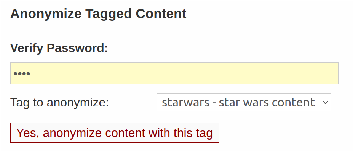
\includegraphics[width=\columnwidth]{figs/lobsters_catanon}
  \end{subfigure}
  \begin{subfigure}[t]{\columnwidth}
  \begin{lstlisting}[language=Ruby,escapeinside={(*}{*)}]
  def tag_anon
    # instantiate the disguise spec with the provided tag to anonymize
    disg_spec = edna.instantiate_spec("tag_anon.json",params[:tag])
    # apply the disguising transformation
    disg_id = edna.apply_disguise(@user.id,params[:passwd],disg_spec)
    # email the disguise ID to the user to allow revealing
    SendDisguiseEmail(@user, disg_id)
  end
  \end{lstlisting}
  \end{subfigure}
  \vspace*{-1em}
    \caption[Hook to invoke topic-based anonymization.]{The Lobsters developer adds a hook in the UI and code to perform
      topic-based anonymization.}
  \label{f:lobsters_hook}
  \end{figure}

%
The Lobsters developer can realize topic-based anonymization as a \xxing
transformation.
%
First, the developer writes a \xx specification that instructs \sys to
decorrelate comments and remove votes on ``Star Wars'' stories
(Figure~\ref{f:spec}).
%
They also add frontend code and UI elements that allow authenticated users to
trigger the \xxing transformation (Figure~\ref{f:lobsters_hook}).
%
When Bea wants to anonymize their contributions on content tagged ``Star Wars,''
Lobsters invokes \sys with the provided specification.

%
Later, if Bea asks Lobsters to deanonymize their ``Star Wars'' contributions, Lobsters
invokes \sys with Bea's reveal credentials and the disguise ID, and \sys reveals
Bea's associations with ``Star Wars'' posts.
%

%%%%%%%%%%%%%%%%%%%%%%%%%%%%%%%%%%%%%%%%%%%%%%%%%%%%%%%%%%%%%%%%
%\section{Design}

\section{Disguise Specifications}
\label{s:spec}

\begin{figure}[t]
\centering
\begin{lstlisting}[style=rust,escapeinside={(*}{*)}]
// Decorrelate comments on stories w/tag {{TAG}}
"comments": [{
  "type": "Decorrelate",
  "predicate": "tags.tag = {{TAG}}",
  "from": "comments JOIN stories ON comments.story_id = stories.id
           JOIN taggings ON stories.id = taggings.story_id
           JOIN tags ON...",
  // decorrelate-specific fields 
  "group_by": "comments.story_id",
  "principal_fk": "comments.user_id" } ],
// Remove votes on stories w/tag {{TAG}}
"votes": [{
  "type": "Remove",
  "predicate": "tags.tag = {{TAG}}",
  "from": "votes JOIN stories...",
}, ... ]
\end{lstlisting}
    \caption[Lobsters topic-based anonymization disguise specification.]{Lobsters topic-based anonymization \xx specification (JSON
    pseudocode), which decorrelates comments and removes votes on stories with
    the specific topic tag.}
\label{f:spec}
\end{figure}


\sys's goal is for developers to reason only about the high-level semantics of
disguising expressed in the disguise specification. \sys takes care of applying
disguise transformations, composing them with other disguising and revealing
transformations, and creating and storing disguised data.


\Xx specifications tell \sys what application data objects to \xx and how to \xx
them.
%
A \xx specification (Figure~\ref{f:spec}) identifies objects to disguise by
database table name and predicate, where a predicate is a SQL \fn{WHERE} clause.
%
By default, \sys \xxs all objects with a foreign-key relationship to 
the principal being disguised\footnote{A
principal refers to an application object representing a user (\eg a row in a
\texttt{users} table). This thesis uses ``principal'' to mean either an 
application object representing a real application client user, or a
pseudoprincipal (a fake application user).},
%, as
%defined by a foreign-key relationship to the principals table, 
but predicates
can narrow the transformation's scope (\eg to stories with specific tags).
%
For each selected group of objects, developers choose to \emph{remove},
\emph{modify}, or \emph{decorrelate} them (\S\ref{s:semantics:spec}).
%, replacing some or all of their contents with placeholder values;
%or \three{} \emph{decorrelate} them.
%where decorrelation removes associations between principals and objects and
%re-associates the objects with pseudoprincipals. \hmng{this is a pretty verabtim
%repetition from section 3, remove or condense I'd say?}
%

The example specification in Figure~\ref{f:spec} decorrelates all comments and
removes all votes on stories with a particular tag, specified by the
\texttt{TAG} parameter provided at invocation time.  The specified foreign key
(\texttt{''principal\_fk''}) for decorrelation of comments tells \sys which
foreign key to the principals table to rewrite. 
%
Decorrelation can use pseudoprincipals at different granularities.  In the
extreme, the \xx specification may tell \sys to create a unique pseudoprincipal
for each decorrelated application object.  In our example, however, all comments
by the same user on the same story decorrelate to the same pseudoprincipal by
setting \verb+"group_by": "comments.story_id"+: for all comments with the same
\texttt{"stories\_id"} value, \sys will rewrite \texttt{"pseudoprincipal\_fk"}
to the same pseudoprincipal identifier.  This allows the application to keep
same-story comment threads intact.
%
\S\ref{s:semantics:spec} describes the semantics of disguise specifications in more
detail.
%
%or a custom set of objects specified by the \xxing transformation.
%\lyt{skipping the ``custom set of objects''; that seems unclear to me.}
%

%%%%%%%%%%%%%%%%%%%%%%%%%%%%%%%%%%%%%%%%%%%%%%%%%%%%%%%%%%%%%%%%%%%%%%%%%%%%%%
\section{User Reveal Credentials}
\sys provides developers and users with the abstraction of \emph{reveal
credentials}, which users provide to the application to authorize revealing
their data.
%
Reveal credentials allow applications that use \sys to support familiar user
authentication workflows when users want to reveal their disguised data. 
%

%
\sys supports two forms of reveal credentials: \one{} the user's private key
itself; or \two{} the user's application password or a recovery token (in case
they forget their password), either of which \sys can use to rederive the
private key.
%
Developers can use either of these credentials depending on application needs.
%
In the Lobsters example, \sys rederives the user's private key using their password.
%
% To support forgetful users, Lobsters could use a backup token.
% secret stored with a third party as a recovery token;
%
% users who forget their passwords would authenticate to this third party to
% retrieve their Lobsters token, and provide it to \sys to rederive the relevant
% private key.
%
Password or keypair changes require an application to re-register the user with
\sys, which generates new recovery tokens and re-encrypts the user's \xxed data.
%
%Alternatively, the application may keep password-encrypted private keys; users
%authenticate with their password to the application, but the application provides the decrypted
%private key to \sys as the reveal credential.
%\sys can thus flexibly support the various common user authorization protocols used by applications
%today.
%
%Users can use their password (the common case), just as they would need to in order to access the
%application.
%
%The application can give the user the backup credential to store locally, or can send it to a
%trusted third party that the user can retrieve from if the user forgets their password.
%
%Finally, the application can simply let the user use their private key directly if they wish.

%
%Using passwords as credentials renders the encryption on the users data only as secure as the user's
%password, but maintains good usability as users can use their application password to reveal data.
%

%%%%%%%%%%%%%%%%%%%%%%%%%%%%%%%%%%%%%%%%%%%%%%%%%%%%%%%%%%%%%%%%%%%%%%
\section{Global Database Updates} 
\label{s:overview:updates}

%\sys allows disguised data to be restored to the database via revealing
%transformations. However, 
Web application databases often undergo global updates 
initiated by an admin or developer, like schema changes or global content
changes (\eg normalizing URLs of all stories). 
%
However, developer updates to the database will fail to apply to any disguised
data at the time. A naive reveal algorithm might incorrectly overwrite these
updates.
%
To ensure updates are applied to revealed data, the developer must inform \sys
about the update so \sys can apply the update to the disguised data when
revealing it.

When a database update is performed, the developer writes a corresponding
\emph{reveal-time update specification} that captures the effects of the
operation and invokes \sys's API with the update specification
(\S\ref{s:semantics:updates}). \sys stores
these update specifications in an \emph{update replay log} that \sys reads upon
reveal in order to apply updates to disguised data before revealing it.
%
%If the developer performs a global application change that \eg normalizes the
%URLs of stories, the developer performs a bulk update in the Lobsters
%applications. The developer also writes an update specification encoding how to
%update individual user's stories' URLs as well. Then the developer invokes
%\sys's \texttt{record\_update} API call with the update.
%

%
%Developers provide \sys with information about updates or schema
%migrations to allow \sys to reveal data without overwriting or conflicting with
%these changes.
%%
%When the developer performs operations that need to hold over revealed
%data---\eg moderations---they will additionally invoke \sys's API, allowing \sys
%to record and appropriately apply updates.
%%

%%%%%%%%%%%%%%%%%%%%%%%%%%%%%%%%%%%%%%%%%%%%%%%%%%%%%%%%%%%%%%%%%%%%%%
\section{Guarantees and Threat Model}
\label{s:threat}
%
%\sys assumes well-intentioned developers who follow standard security practices
%(\eg password protections)
%and write \xx specifications that capture the desired application semantics.
%
%\sys \xxs data according to these specifications, but because the database
%retains some data,
%to keep application semantics intact,
%\sys cannot protect against statistical correlation attacks.
%provide information-theoretic privacy guarantees.
%
%Developers and users can reason about the security properties of disguised data given \sys's
%threat model.
\sys protects the confidentiality of \xxed data between the time when a user
disguises their data and the time when they reveal it.
%
%(where \xxed data is defined by the trusted developer-provided disguise specification).
%
During this period, \sys ensures that the application can neither learn the contents of
disguised data, nor what \xxed data corresponds to which user, even if the
application is compromised and an attacker dumps the database contents (\eg via
SQL injection).
%
\sys encrypts \xxed data, so its confidentiality stems from ``crypto
shredding,'' an approach based on the fact that ciphertexts are
indistinguishable from garbage data if the key material is
unavailable~\cite{dnefs,townsend:cryptoshredding,aws:cryptoshredding,gtr:cryptoshredding}.\footnote{Crypto
shredding assumes sufficiently random key material; for usability, \sys allows 
users to either provide a private key or their password as credentials, which
weakens \sys's guarantees.}
%

% STANDARD CLAIMS ABOUT CRYPTO ASSUMPTIONS
%
We make standard assumptions about the security of cryptographic primitives:
attackers cannot break encryption, and keys stored with clients are safe.
%
If a compromised application obtains a user's credentials, either because the
user provides them to the application for reveal, or via external means such as
phishing, \sys provides no guarantees about the user's current or future
disguised data.
%
\sys also expects the application to protect backups created prior to
disguising. External copies of the data (\eg Internet Archive or screenshots)
are out of scope.
%

%
While \sys hides the contents of \xxed data and relationships between \xxed data
and users, it does not hide the existence of
\xxed data. (An attacker can see if
a user has \xxed some data, but cannot see which \xxed data corresponds to this
user.)
%
An attacker can also see any data left in the database, such as pseudoprincipal
data or embedded text.
%
\sys puts out of scope attacks that leverage this leftover data
and metadata to infer which principal originally owned which objects.
%

\sys's choice of threat model and its limitations stem from
\sys's goal of practicality and usability by existing applications.
%
For example, decorrelation with pseudoprincipals removes explicit user-content
links, but leaves placeholder information in the database to avoid application
code having to handle dangling references.
%
Similarly, leveraging server-side storage to hold \xxed data leaves
metadata available to attackers, but avoids burdening users with data storage
management.
%
We believe a stronger threat model would require greater modification of
existing applications.
